%% Für Bindekorrektur als optionales Argument "BCORfaktormitmaßeinheit", dann
% sieht auch Option "twoside" vernünftig aus
% Näheres zu "scrartcl" bzw. "scrreprt" und "scrbook" siehe KOMA-Skript Doku
\documentclass[12pt,a4paper,titlepage,headinclude,bibtotoc]{scrartcl}


%---- Allgemeine Layout Einstellungen ------------------------------------------

% Für Kopf und Fußzeilen, siehe auch KOMA-Skript Doku
\usepackage[komastyle]{scrpage2}
\pagestyle{scrheadings}
\setheadsepline{0.5pt}[\color{black}]

\usepackage{amsmath}

\usepackage{floatflt}

\setlength{\parindent}{0pt}

\usepackage{listings}

\usepackage{float}

\usepackage{dsfont} 

%Einstellungen für Figuren- und Tabellenbeschriftungen
\setkomafont{captionlabel}{\sffamily\bfseries}
\setcapindent{0em}

%---- Weitere Pakete -----------------------------------------------------------
% Die Pakete sind alle in der TeX Live Distribution enthalten. Wichtige Adressen
% www.ctan.org, www.dante.de

% Sprachunterstützung
\usepackage[ngerman]{babel}

% Benutzung von Umlauten direkt im Text
% entweder "latin1" oder "utf8"
\usepackage[utf8x]{inputenc}
%\usepackage[utf8]{inputenc}

% Pakete mit Mathesymbolen und zur Beseitigung von Schwächen der Mathe-Umgebung
\usepackage{latexsym,exscale,stmaryrd,amssymb,amsmath}

% Weitere Symbole
\usepackage[nointegrals]{wasysym}
\usepackage{eurosym}

% Anderes Literaturverzeichnisformat
%\usepackage[square,sort&compress]{natbib}

% Für Farbe
\usepackage{color}

\usepackage{graphicx}

\usepackage[euler]{textgreek}

\usepackage{wrapfig}

\usepackage{subfigure}

\usepackage{sidecap}

% Befehl für "Entspricht"-Zeichen
\newcommand{\corresponds}{\ensuremath{\mathrel{\widehat{=}}}}

%Für chemische Formeln (von www.dante.de)
%% Anpassung an LaTeX(2e) von Bernd Raichle
\makeatletter
\DeclareRobustCommand{\chemical}[1]{%
  {\(\m@th
   \edef\resetfontdimens{\noexpand\)%
       \fontdimen16\textfont2=\the\fontdimen16\textfont2
       \fontdimen17\textfont2=\the\fontdimen17\textfont2\relax}%
   \fontdimen16\textfont2=2.7pt \fontdimen17\textfont2=2.7pt
   \mathrm{#1}%
   \resetfontdimens}}
\makeatother

\definecolor{source_green}{rgb}{0,0.6,0}
\definecolor{source_gray}{rgb}{0.5,0.5,0.5}
\definecolor{source_mauve}{rgb}{0.58,0,0.82}

\lstset{
  language=C++,                % choose the language of the code
  numbers=left,                   % where to put the line-numbers
  stepnumber=1,                   % the step between two line-numbers.        
  numbersep=5pt,				% how far the line-numbers are from the code
  basicstyle=\scriptsize,                  
  backgroundcolor=\color{white},  % choose the background color. You must add \usepackage{color}
  showspaces=false,               % show spaces adding particular underscores
  showstringspaces=false,         % underline spaces within strings
  showtabs=false,                 % show tabs within strings adding particular underscores
  tabsize=2,                      % sets default tabsize to 2 spaces
  captionpos=b,                   % sets the caption-position to bottom
  breaklines=true,                % sets automatic line breaking
  inputencoding=utf8,
   extendedchars=true,
   literate={á}{{\'a}}1 {ã}{{\~a}}1 {é}{{\'e}}1,
  keywordstyle=\color{blue},
  numberstyle=\tiny\color{source_gray},
  stringstyle=\color{source_mauve},
  commentstyle=\color{source_green},
  breakatwhitespace=true,         % sets if automatic breaks should only happen at whitespace
  title=\lstname,                 % show the filename of files included with \lstinputlisting;
}


\usepackage{textcomp}
\usepackage{pdfpages}

\begin{document}
%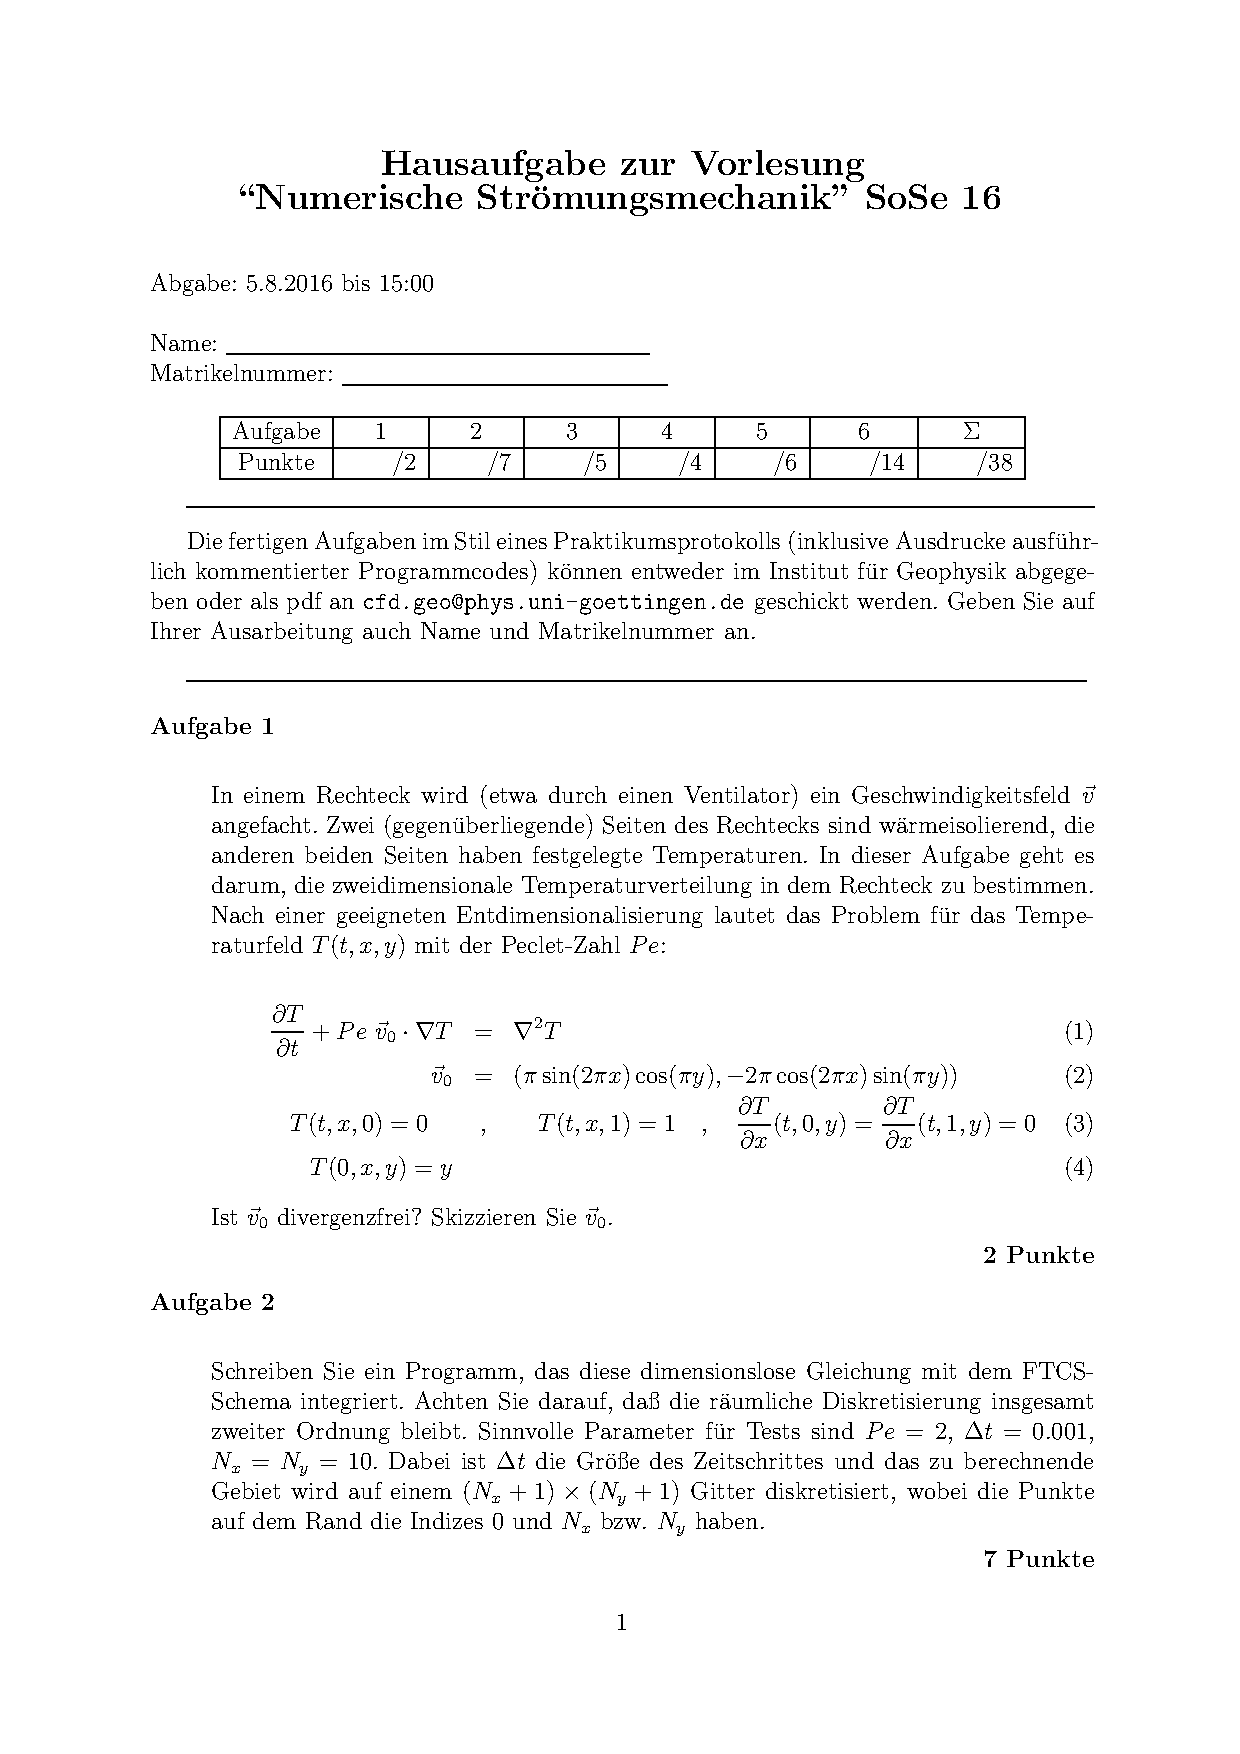
\includepdf[pages={1-3}]{task.pdf}
%\setcounter{page}{1}

\begin{titlepage}
\centering
\textsc{\Large \\
[1.5ex]Georg-August-Universität Göttingen Sommersemester 2016}

\vspace*{2.2cm}

\rule{\textwidth}{1pt}\\[0.5cm]
{\large \bfseries
  Hausarbeit zur Vorlesung\\[1.5ex]
  \huge Numerische Strömungsmechanik}
\rule{\textwidth}{1pt}

\vspace*{1.0cm}

\begin{figure}[H]  
	\centering
   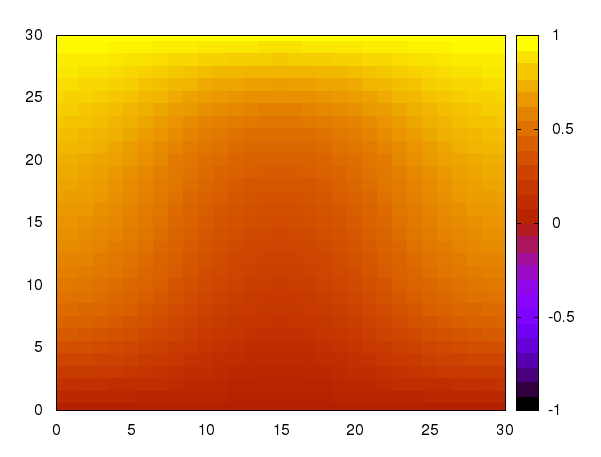
\includegraphics[width=0.7\textwidth]{res/title/2_05.png}
\end{figure}

\begin{Large}
\begin{tabular}{ll}
Name: & Roland Zimmermann\\
Matrikelnummer:	& 21426901 \\
Mail Adresse: & roland.zimmermann@stud.uni-goettingen.de \\ 
Abgabetermin: & 05.08.2016\\
\end{tabular}
\end{Large}

\end{titlepage}



\tableofcontents

\newpage

\section{Einleitung}
\label{sec:einleitung}
Viele Verhaltensweisen und Effekte in der Natur können durch partielle Differenzialgleichungen beschrieben werden. Die Lösung dieser ist allerdings nur in wenigen, speziellen Fällen analytisch möglich. Für die restlichen Fälle müssen numerische Lösungsverfahren verwendet werden. Gerade diese Szenarien spielen beispielsweise in der Auto- und Luftfahrtindustrie eine relevante Rolle bei der Produktentwicklung und Optimierung. In dieser Arbeit werden, hierdurch motiviert, zwei verschiedene Lösungsverfahren für ein solches Problem implementiert und anschließend analysiert.

\section{Fragestellung}
\label{sec:fragestellung}
In dieser Hausaufgabe wird die Wärmeausbreitung (siehe \ref{sec:diff_adv}) in einem zweidimensionalen, rechteckigen System betrachtet. Diese soll durch ein extern erzeugtes Geschwindigkeitsfeld (beispielsweise durch einen Ventilator) verstärkt werden. Dieses Vektorfeld soll nicht zeitabhängig sein, und lässt sich in dimensionsloser Form durch
\begin{align*}
\vec{v} = (\pi \sin(2\pi x) \cos(\pi y), -2 \pi \cos(2\pi x) \sin(\pi y))^t
\end{align*}
beschreiben. Das zu betrachtende System ist ein Quadrat $[0,1]^2$. Für dieses gibt es für jeden der vier Ränder je eine Randbedingung. So soll die Temperatur auf dem oberen Rand $T=1$ und auf dem unteren $T=0$ betragen. An dem linken und rechten Rand soll dagegen die jeweilige Normalenableitung verschwinden. Dies wird durch eine wärmeisoliernde Wand in dem System bedingt. Zu Beginn soll eine Temperaturverteilung der Form $T_{start}(x, y) = y$ vorliegen.\\

Zur Untersuchung des System fallen mehrere Aufgaben an. So wird zuerst das Geschwindigkeitsfeld selber auf seine Divergenz untersucht (siehe \ref{sec:task1}). Anschließend wird eine erste numerische Lösung des Problems (im \textit{FTCS-Schema}) durchgeführt (siehe \ref{sec:task2}). Daraufhin wird nun die numerische Korrektheit dieser Lösung untersucht (siehe \ref{sec:task3}). Schließlich werden für verschiedene Parameter Simulationen durchgeführt, um unter anderem die Stabilität zu beurteilen (siehe \ref{sec:task4}, \ref{sec:task5}). Schließlich wird das Problem noch einmal gelöst, diesmal aber im \textit{BTCS-Schema} (siehe \ref{sec:task6}).\\
Abschließend wird noch ein kurzer Vergleich der beiden Verfahren hinsichtlich ihrer Resultate und der benötigten Rechenzeit durchgeführt.\\
Alle hierfür benötigten Programme und Hilfsroutinen werden in \textit{C++} implementiert.

\section{Theorie}
\label{sec:theorie}
\subsection{Die Diffusions-Advektion-Gleichung}
\label{sec:diff_adv}
Die Ausbreitung von Flüssigkeiten, Gasen beziehungsweise von Energie kann zum einen durch die \textit{Diffusionsgleichung} [3, S.49ff]
\begin{align}
\label{eq:diff}
\frac{\partial}{\partial t}T = D \nabla^2 T 
%= D \left(\frac{\partial^2}{\partial x^2} + \frac{\partial^2}{\partial y^2} \right)T
\end{align}


und zum anderen durch die \textit{Advektionsgleichung}

\begin{align}
\label{eq:adv}
\frac{\partial}{\partial t}T = - \nabla \cdot (\vec{v}\cdot T)
\end{align}
beschrieben werden. Hierbei stehen $T$ für die Verteilung der Energie (Temperatur), $t$ für die Zeit und $D$ für die Diffusionskonstante.
Während die \textit{Diffusionsgleichung} die zeitliche Ausbreitung der Partikel beziehungsweise der Energie, bedingt durch zufällige Bewegungen, beschreibt, beschreibt die \textit{Advektionsgleichung} den Partikelfluss der durch ein Geschwindigkeitsfeld herbeigeführt wird.\\
Fasst man diese beiden Effekte aus den Gleichungen (\ref{eq:adv}) und (\ref{eq:diff}) zusammen [3, S.140ff], so erhält man die \textit{Diffusions-Advektion-Gleichung}
\begin{align*}
\frac{\partial}{\partial t}T = D \nabla^2 T - \nabla \cdot (\vec{v}\cdot T)
%= D \left(\frac{\partial^2}{\partial x^2} + \frac{\partial^2}{\partial y^2} \right)T - (\frac{\partial}{\partial x} + \frac{\partial}{\partial y}) (\vec{v}\cdot T).
\end{align*}
Hierbei kann nun, wenn ein gegebenen externes, divergenzfreies Geschwindigkeitsfeld gegeben ist, dieses aus der Divergenz herausgelöst werden, sodass sich
\begin{align}
\label{eq:orig_diff_adv}
\frac{\partial}{\partial t} T + \vec{v} \cdot \nabla T = D \nabla^2 T
\end{align}
ergibt.\\
Durch das Einführen der \textit{Péclet-Zahl}
\begin{align*}
Pe = \frac{L v \rho c_p}{\lambda}
\end{align*}
ist eine Entdimensionalisierung der Gleichung (\ref{eq:orig_diff_adv}) möglich. Hierbei stehen $L$ für eine charakteristische Länge, $v$ für eine Geschwindigkeit, $\rho$ für die Dichte, $c_p$ für die spezifische Wärmekapazität und $\lambda$ für die Wärmeleitfähigkeit des jeweiligen Mediums. Somit ergibt sich
\begin{align}
\label{eq:diff_adv}
\frac{\partial}{\partial t} T + Pe \cdot \vec{v} \cdot \nabla T = \nabla^2 T.
\end{align}

\subsection{Das FTCS-Schema}
\label{sec:ftcs}
Eine mögliche Methode zur Lösung einer solchen partiellen Differenzialgleichung ist durch die Verfahrensgruppe der finiten Differenzen gegeben. Eine hierfür geeignete Diskretiserung des Problems ist in Form eines \textit{FTCS}-Schemas (Forward in Time, Centered in Space) gegeben. Hierbei wird der Raum in der $x$-Richtung in $(N_x+1)$ und in der $y$-Richtung in $(N_y+1)$ Stützstellen unterteilt, sodass sich ein zweidimensionales räumliches Gitter ergibt. Zwischen diesen Punkten herrscht ein jeweiliger Abstand von $\Delta x = X/N_x$ und $\Delta y = Y/N_y$, wobei $X$ und $Y$ für die Ausmaße des zu beschreibenden Problems in der $x$- und $y$-Richtung stehen.\\
Die Temperatur $T(x, y)$, die hiermit beschrieben werden soll, geht dadurch in die Form $T_{i,j}$ über, wobei $i$ der Index des Punktes in der $x$- und $j$ der in der $y$-Richtung ist. Diese Indizes laufen von $0$ bis $N_x$ beziehungsweise $N_y$.\\
Um nun noch die Zeit zu erfassen, wird auch diese in Punkte diskretisiert, die einen Abstand $\Delta_t$ haben, sodass sich insgesamt ein dreidimensionaler Würfel ergibt, dessen verschiedenen Ebenen für die verschiedenen Zeitpunkte stehen. Erneut geht die Temperatur $T(t, x, y) = T_{i,j}(t)$ über in $T_{i,j}^N$, wobei $N$ für den zeitlichen Index steht. Auch hier wird von $0$ an indiziert.\\

Diese Aufteilung erlaubt es nun, die in den Gleichung (\ref{eq:diff_adv}) vorkommenden Ableitungen zu beschreiben.   
Hierbei wird in dem \textit{FTCS}-Schema die zeitliche Ableitung in der ersten und die räumlichen in der zweiten Ordnung beschrieben. Die Ordnung gibt hierbei jeweils an, wie stark der Fehler von der jeweiligen Schrittweite abhängt. Bei einem Verfahren zweiter Ordnung [1, S.18ff] hängt dieser Fehler von $\mathcal{O}(\Delta x^2)$ ab.
Es ergibt sich für die Ableitungen
\begin{align}
\frac{\partial}{\partial t}T(x,y) &= \frac{T_{i,j}^{N+1} - T_{i,j}^{N}}{\Delta t}, \\
\frac{\partial}{\partial x}T(x,y) &= \frac{T_{i+1,j}^{N} - T_{i-1,j}^{N}}{2 \Delta x}, \\
\frac{\partial^2}{\partial x^2}T(x,y) &= \frac{T_{i+1,j}^{N} - 2 T_{i,j}^{N} + T_{i-1,j}^{N}}{ \Delta x^2}.
\end{align}

Durch Einsetzen in die Gleichung (\ref{eq:diff_adv}) und Umstellen nach $T_{i,j}^{N+1}$ erhält man schließlich %in der zweiten räumlichen Ordnung
\begin{align}
\label{eq:ftcs}
T_{i,j}^{N+1} = T_{i,j}^N &+ \Delta t \left[ -Pe \left( v^x_{i,j} \frac{T_{i+1,j}^N-T_{i-1,j}^N}{2\Delta x}+v^y_{i,j} \frac{T_{i,j+1}^N-T_{i,j-1}^N}{2\Delta x} \right) \right. \nonumber \\ 
 & \left.+ \frac{ T_{i+1,j}^N - 2 T_{i,j}^N +  T_{i-1,j}^N }{\Delta x^2} 
+ \frac{ T_{i,j+1}^N - 2  T_{i,j}^N + T_{i,j-1}^N}{\Delta y^2} \right],
\end{align}
womit die Integration durchgeführt werden kann. Die Ausdrücke $v^x_{i,j}$ und $v^y_{i,j}$ stehen für die jeweilige $x$- und $y$-Komponente des zeitlich konstanten Geschwindigkeitsfeldes an dem jeweiligen Ort.\\
Des Weiteren sind allerdings noch die Randbedingungen zu beachten. Hierbei muss die Differenzialgleichung besonders betrachtet werden, da hier nur Nachbarpunkte in eine Richtung existieren.\\
Bei den \textit{Dirichlet}-Rändern können die Werte am Rand konstante gehalten werden, sodass
\begin{align*}
T^{N+1}_{Rand} = T^{N}_{Rand} \Rightarrow T^{N+1}_{i,0} = T^{N}_{i,0} = 0 \land T^{N+1}_{i,N_y} = T^{N}_{i,N_y} = 1
\end{align*}
eine geeignete mathematische Beschreibung ist. Exemplarisch für die \textit{Neumann}-Ränder wird der linke Rand betrachtet, auf dem die erste Ableitung in $x$-Richtung verschwinden soll. Durch eine Taylor-Entwicklung und einen Koeffizientenvergleich erhält man die diskretisierte Randbedingung zweiter Ordnung
\begin{align*}
T_{0,j}^{N+1} - \frac{4}{3} T_{1,j}^{N+1} + \frac{1}{3} T_{2,j}^{N+1} = 0.
\end{align*}
In diesem Problem muss eine analoge Gleichung auch noch für den rechten Rand betrachtet werden.

\subsection{Das BTCS-Schema}
\label{sec:btcs}
Ein alternativer Ansatz zur Lösung ist das \textit{BTCS}-Schema (Backward in Time, Centered in Space), bei der räumlich erneut eine Diskretisierung zweiter Ordnung durchgeführt wird, diese allerdings zum Zeitpunkt $(N+1)$ ausgewertet wird [3, S.170ff]. Zeitlich wird auch wieder ein Verfahren erster Ordnung verwendet.
Somit ergibt sich der Ausdruck
\begin{align}
\label{eq:impli}
T_{i,j}^{N} = \alpha T_{i,j}^{N+1} + \beta^-_{i,j} T_{i-1,j}^{N+1} + \beta^+_{i,j} T_{i+1,j}^{N+1} + \gamma^-_{i,j} T_{i,j-1}^{N+1} + \gamma^+_{i,j} T_{i,j+1}^{N+1}.
\end{align}
Dabei wurden die folgenden Abkürzungen eingeführt und benutzt
\begin{align*}
\alpha &= \Delta t \left(\frac{2}{\Delta x^2} + \frac{2}{\Delta y^2} + \frac{1}{\Delta t} \right), \\
\beta^\pm_{i,j} &= \Delta t \left(-\frac{1}{\Delta x^2} \pm \frac{Pe v^x_{i,j}}{2 \Delta x}\right), \\
\gamma^\pm_{i,j} &= \Delta t \left(-\frac{1}{\Delta y^2} \pm \frac{Pe v^y_{i,j}}{2 \Delta y}\right).
\end{align*}
Dies gilt allerdings nur für die inneren Punkte des Gitters. Für den linken und rechten Rand gelten, um ebenfalls die Diskretisierung in der zweiten Ordnung umsetzen zu können, die Gleichungen
\begin{align}
\label{eq:impli_neumann_l}
T^{N+1}_{0,j} - \frac{4}{3} T^{N+1}_{1,j} + \frac{1}{3} T^{N+1}_{2,j} &= 0, \\
\label{eq:impli_neumann_r}
T^{N+1}_{N_x,j} - \frac{4}{3} T^{N+1}_{N_x-1,j} + \frac{1}{3} T^{N+1}_{N_x-2,j} &= 0.
\end{align}

Um das Problem nun besser beschreiben zu können, wird das zweidimensionale Feld in einem eindimensionalen Spaltenvektor zusammengefasst. Hierfür ist es notwendig, die Indizes umzubenennen. Hierbei wird ab jetzt die folgende Konvention benutzt: durchlaufe erst alle $x$-Werte zu einem festen $y$-Wert, und erhöhe den $y$-Wert. Dies bewirkt, dass die Zeilen des Feldes hintereinander geschrieben werden:
\begin{align*}
T_{i,j}^{N} = T_{i+N_y j}^{N}.
\end{align*}
Nun kann die Gleichung (\ref{eq:impli}) als eine Matrixoperation der Form
\begin{align*}
\vec{F} = M \cdot \vec{T}^{N+1},
\end{align*} 
mit der Matrix \textbf{M} ausgedrückt werden. Hierbei geht $\vec{F}$ aus $\vec{T^N}$ hervor, wobei einige Einträge auf null gesetzt werden, um die Gleichungen (\ref{eq:impli_neumann_l}) und (\ref{eq:impli_neumann_r}) korrekt als Matrix-Gleichung darzustellen.
Die Matrix \textbf{M} hat fünf Diagonalen, die ungleich null sind. \textbf{M} kann nun als Blockmatrix
\begin{align*}
\boldsymbol{M} = \begin{pmatrix}
  \mathds{1}  & 0 & 0 &  0 & . & . & . & . & 0 \\
  E^-  & D & E^+ &  0 & . & . & . & . & 0 \\
  0  & E^- & D & E^+ & 0 &  . & . & . & 0\\
  . & & . & . & . & & & &  . \\
  . & & & . & . & . & & &  . \\
  . & & & &  . & . & . & &  . \\
  . & &  & & &  . & . & . &  . \\
  .  & . & . & . & . & 0 & E^- & D & E^+ \\
  0  & . & . & . & . & . & . & . & \mathds{1} \\
 \end{pmatrix}
,
\end{align*}
mit den quadratischen Matrizen $\textbf{E}^\pm$, \textbf{D} und der Einheitsmatrix $\mathds{1}$ geschrieben werden. Die beiden Einheitsmatrizen im oberen linken und unteren rechten Eck setzen hierbei die \textit{Dirichlet}-Randbedingungen am oberen und rechten Rand um.
Die Matrizen \textbf{D} und $\textbf{E}^\pm$ 

\begin{align*}
\boldsymbol{E^\pm} = \begin{pmatrix}
	0 & . & .& .& .& 0\\
	. & \gamma^\pm & . & . & . & .\\
	. & 0 & \gamma^\pm & 0 & . & .\\
	. & . & 0 & \gamma^\pm & 0  & .\\  
	. & . & . & 0 &  \gamma^\pm & .\\ 
	0 & . & .& .& .& 0\\
 \end{pmatrix}
\end{align*}
\begin{align*}
 \boldsymbol{D} = \begin{pmatrix}
	1 & -\frac{4}{3} & \frac{1}{3} & .& .& 0\\
	\beta^- & \alpha & \beta^+ & 0 &  & .\\ 
	0 & \beta^- & \alpha & \beta^+ & 0 & .\\ 
	. & . & \beta^- & \alpha & \beta^+ & 0\\ 
	. &   & 0 & \beta^- & \alpha & \beta^+\\ 
	0 & . & .& \frac{1}{3} & -\frac{4}{3} & 1\\
 \end{pmatrix}.
 \end{align*}
 setzen die implizite Gleichungen (\ref{eq:impli}) und (\ref{eq:impli_neumann_l}) um, sind also das Kernstück des \textit{BTCS-Schemas}. Ihre erste und letzte Zeile weichen hierbei vom Rest ab, da sie die \textit{Neumann}-Randbedingungen umsetzen.
Um das System nun um einen Zeitschritt weiter zu simulieren, muss die Matrix $\textbf{M}$ invertiert werden - beziehungsweise das Gleichungssystem $\textbf{M} \vec{x} = \vec{b}$ gelöst werden.\\
Hierfür hat sich das \textit{SOR-Verfahren} (Successive Over-Relaxation), welches eine Modifikation des \textit{Gauß-Seidel-Verfahrens} ist, als besonders geeignet herausgestellt. Dies sind beides iterative Lösungsverfahren. Um sie verwenden zu können, wird die Matrix zuerst in drei Teilmatrizen $\boldsymbol{M}=\boldsymbol{L}+\boldsymbol{D}+\boldsymbol{U}$ zerlegt, wobei $D$ eine Diagonal-, $L$ eine untere Dreiecks- und $U$ eine obere Dreiecksmatrix ist. Zudem wird der \textit{Residuen-Vektor} $\vec{r_n} = \boldsymbol{M} \vec{x_n} - \vec{b}$ eingeführt, wobei der Index den jeweiligen Iterationsschritt angibt. Dieser Vektor beschreibt die Differenz zwischen der korrekten und der iterativen Lösung der Gleichung $\boldsymbol{M} \vec{x} = \vec{b}$.\\
Durch diese Zerlegung ist es möglich eine rekursive Bestimmungsformel [2, S. 25ff]
\begin{align*}
\vec{x}^{\,n} = \vec{x}^{\,n-1} - \alpha(\boldsymbol{L}+\boldsymbol{D})^{-1} \vec{r}^{\,n-1}
\end{align*}
aufzustellen. Hierbei ist $\alpha$ der so genannte \textit{Relaxationsparameter}, welcher bei dem \textit{Gauss-Seidel-Verfahren} gleich eins ist.\\
Diese Matrizen-Gleichung kann in Summenschreibweise durch Eigenschaften triagonaler Matrizen aus der linearen Algebra auch als
\begin{align}
\label{eq:sor}
x^{n+1}_i = (1-\alpha)x^{n}_i + \frac{\alpha}{m_{i,i}} \left(b_i - \sum\limits_{j=1}^{i-1} m_{i,j} x^{n+1}_j - \sum\limits_{j=i+1}^{N} m_{i,j} x^{n}_j \right)  
\end{align}
aufgefasst werden [2, S.30], wobei $N$ die Dimensionen des Problems angibt.

\section{Durchführung der Aufgaben}
\subsection{Aufgabe 1: Untersuchung von $\vec{v}$}
\label{sec:task1}
Für die numerische Betrachtung des Problems spielt der Einfluss von $\vec{v}$ eine entscheidende Rolle. Ist dieses Geschwindigkeitsfeld nämlich divergenzfrei, so ergibt sich eine mögliche, vereinfachende Betrachtung in diskretisierter Form nach Gleichung (\ref{eq:ftcs}). Für das externe Feld
\begin{align*}
\vec{v} = (\pi \sin(2\pi x) \cos(\pi y), -2 \pi \cos(2\pi x) \sin(\pi y))^t
\end{align*}
gilt
\begin{align*}
\nabla \cdot \vec{v} = \frac{\partial}{\partial x} \left(\pi \sin(2\pi x) \cos(\pi y)\right) + \frac{\partial}{\partial y} \left(-2 \pi \cos(2\pi x) \sin(\pi y)\right) = 0;
\end{align*}
es ist somit divergenzfrei. Es bietet sich zudem an, das Feld grafisch darzustellen. Dies kann in Abbildung (\ref{fig:task1}) nachvollzogen werden.
\begin{figure}[H]
 \centering
   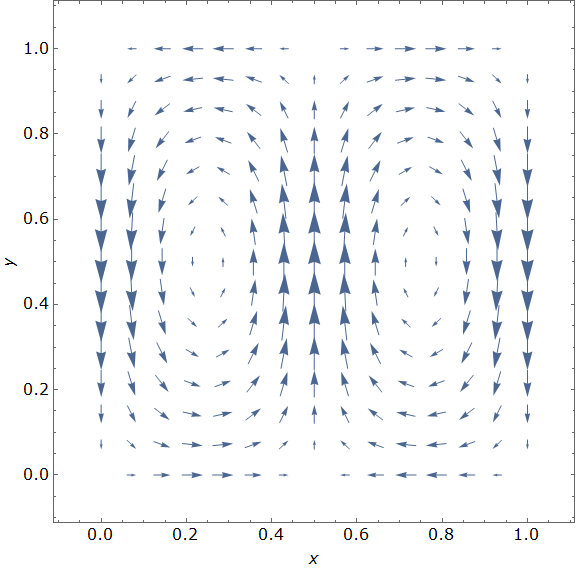
\includegraphics[width=0.6\textwidth]{res/task1.png}
   \caption{Grafische Darstellung des Geschwindigkeitsfeldes $\vec{v}$ in Abhängigkeit von $x$ und $y$.}
 \label{fig:task1}
\end{figure}
Es ist zu erkennen, dass das Feld zwei Zentren hat, um die sich je ein Strudel bildet. Diese laufen in der Mitte zusammen, und strömen zum oberen Rand hin.

\subsection{Aufgabe 2: FTCS-Lösung}
\label{sec:task2}
Um nun eine erste numerische Lösung erzeugen zu können, wird das zuvor in (\ref{sec:ftcs}) hergeleitete Verfahren benutzt. Hierfür wird direkt eine etwas allgemeinere Implementation gewählt, welche in der Integration auch mögliche Quellterme berücksichtigt. Dieser Ansatz wird gewählt, da im weiteren Verlauf dieser Arbeit (siehe \ref{sec:task3}) die numerische Korrektheit des Integrators überprüft werden soll. Hierfür wird eine Quelle hinzugefügt, welche eine analytische Lösung erlaubt.\\
Das Programm aus Quellcode (1) besteht aus zwei verschiedenen Routinen. Die \textit{main}-Methode liest ge-wünschte Eingangsparameter, wie die Schrittweite $\Delta t$, die maximale Integrationszeit $t_{max}$, die \textit{Péclet-Zahl} $Pe$, die Gitterauflösung $N_x$ und $N_y$ und einen weiteren Parameter, der angibt, ob ein Quellterm erzeugt werden soll, ein (Zeile 78-119). Zudem erzeugt sie Objekte des Types \textsc{vector\textless vector\textless double\textgreater \textgreater}, in welchem der Temperaturverlauf in dem Rechteck, und ein etwaiger Quellterm abgespeichert werden. Hierfür wird ein \textsc{vector} statt eines Feldes genutzt, um mögliche \textsc{Acess Violation Exceptions} zu vermeiden und um Memoryleaks zu reduzieren (Zeile 121-163). Etwaige Leistungsverluste hierdurch sind zum einen begrenzt und steuern keinen großen Anteil zu der Gesamtlaufzeit bei.\\
In einer Schleife wird in den gewählten Zeitschritten bis zur Endzeit iteriert, und für jede Zeit ein Integrationsschritt durchgeführt (Zeile 131-163). Im Anschluss daran wird die benötigte Rechenzeit ausgegeben (Zeile 165-166 und 202-205). Zuletzt wird die berechnete Temperaturverteilung in die vorher angegebene Datei ausgegeben (Zeile 208-215).\\
Der jeweilige Integrationsschritt wird von der \textit{ftcs\_time\_step}-Methode ausgeführt. Diese legt zuerst eine Kopie des übermittelten Feldes an, um auf Grundlage dieser, die Ableitungsterme berechnen zu können. Hierfür wird in einer Schleife über das gesamte Gitter iteriert, und jeweils der $\nabla^2 T$ und der $\vec{v_0} \cdot \nabla T$ Term einzeln berechnet und anschließend nach Gleichung (\ref{eq:ftcs_source}) als Änderung von $T$ verrechnet (Zeile 19-59). Abschließend werden noch die \textit{Dirichlet}- und \textit{Neumann}-Ränder beachtet und die Werte passend aktualisiert (Zeile 61-76). 

\subsection{Aufgabe 3: Numerische Korrektheit der FTCS-Lösung}
\label{sec:task3}
Zur Beurteilung der Korrektheit der numerischen Lösung wird normalerweise erstmal versucht, das Ergebnis mit der analytischen Lösung zu vergleichen. Da dieses Problem allerdings nicht analytisch lösbar ist, muss hier anders verfahren werden. Als Ansatz hierbei wird eine mögliche stationäre Lösung geraten, und die Differenzialgleichung um einen Quellterm so ergänzt, dass dies die exakte Lösung des Problems ist.\\
Für diese konstruierte stationäre Lösung wird der Ansatz
\begin{align*}
T^* = \cos(\pi x) \sin(\pi y) + y
\end{align*} 
gewählt, da dies die vier Randbedingungen erfüllt.
Um den Quellterm $Q$ zu korrigieren, wird $T^*$ in die stationäre Gleichung
\begin{align*}
Pe \cdot \vec{v} \nabla T^* = \nabla^2 T^* + Q 
\end{align*}
eingesetzt, welche auch Quellen berücksichtigt. Es ergibt sich somit
\begin{align*}
Q = Pe \cdot \vec{v} \nabla T^* - \nabla^2 T^*,
\end{align*}
was sich nach Einsetzen des Ansatzes und des gegebenen Geschwindigkeitsfeldes zu
\begin{align*}
Q = \pi^2 \left(2 \cos(\pi x) \sin(\pi y) - Pe \cdot \cos(\pi x)^3 \sin(2 \pi y) \right) - 2 Pe \cdot \pi \cos(2 \pi x) \sin(\pi y)
\end{align*}
ergibt.\\
Berücksichtigt man diesen Quellterm in dem \textit{FTCS-Schema}, folgt:
\begin{align}
\label{eq:ftcs_source}
T_{i,j}^{N+1} = T_{i,j}^N & + \Delta t \left[ -Pe \left( v^x_{i,j} \frac{T_{i+1,j}^N-T_{i-1,j}^N}{2\Delta x}+v^y_{i,j} \frac{T_{i,j+1}^N-T_{i,j-1}^N}{2\Delta x} \right) \right. \nonumber \\ 
 & \left.+ \frac{ T_{i+1,j}^N - 2 T_{i,j}^N +  T_{i-1,j}^N }{\Delta x^2} 
+ \frac{ T_{i,j+1}^N - 2  T_{i,j}^N + T_{i,j-1}^N}{\Delta y^2} + Q_{i,j} \right],
\end{align}

Die Berechnung und Zuweisung dieses Quellterms (Zeile 148-161) wurde im Quellcode (1) implementiert. 
Nun kann zu jedem Zeitpunkt die Differenz zwischen der stationären Lösung $T_{i,j}^*$ und der numerischen Lösung $T_{i,j}^N$ berechnet werden als
\begin{align*}
\sigma^N = \sqrt{\Sigma_{i,j} (T_{i,j}^N - T_{i,j}^*)^2 }.
\end{align*}
Diese Abweichung wird nun alle $100$ Zeitschritte in der \textit{main}-Methode (Zeile 175-196) ausgegeben.\\
Setzt man nun noch $N_x = N_y$, und variiert diese Werte für ein festes $\Delta t$, so können Aussagen getroffen werden, über die Abweichungen der stationären numerischen $T$ und der tatsächlichen stationären Lösung $T^*$ in Abhängigkeit von der Gittergröße.

\begin{figure}[H]
 \centering
   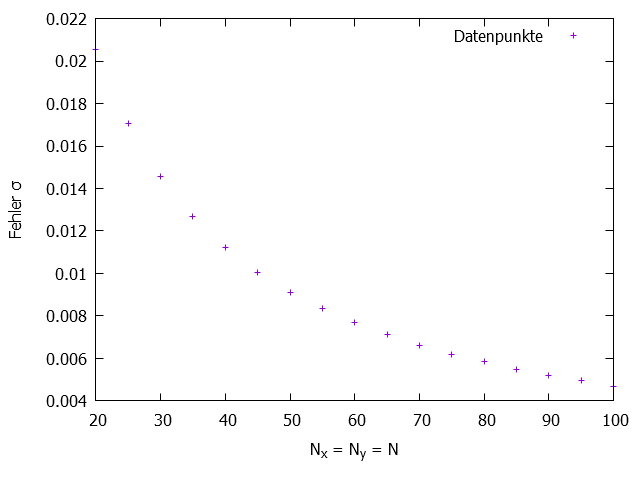
\includegraphics[width=0.7\textwidth]{res/task3.png}
   \caption{Grafische Auftragung der numerischen Abweichung $\sigma$ in Abhängigkeit von der Gittergröße $N$.}
 \label{fig:task3}
\end{figure}

In Abbildung (\ref{fig:task3}) zeigt den Verlauf des Fehlers $\sigma$ in Abhängigkeit von $N_x = N_y$ für $Pe = 2$ für einen Zeitschritt von $\Delta t = 2 \cdot 10^{-5}$ aufgetragen.
Zudem wurde eine eine Regression durchgeführt, welche eine Abhängigkeit der Form $\sigma = N^{-1.2}$ ergeben hat. Dazu ist noch anzumerken, dass für größere $N$-Werte (größer als $115$) der Fehler nicht mehr weiter sinkt, sondern sogar stark anwächst, da die numerische Lösung divergent wird.


\subsection{Aufgabe 4: Auswertung verschiedener FTCS-Lösungen}
\label{sec:task4}
Im weiteren Verlauf wird der zuvor eingeführte Quellterm $Q=0$ gesetzt. Nun kann das Temperaturfeld $T$ für zwei verschiedene \textit{Péclet-Zahlen} $Pe = 2$ und $Pe = 10$ simuliert,
und zu den drei Zeitpunkten $t = 0.005$, $t = 0.05$ und $t=0.5$ visualisiert werden. Hierfür wird $\Delta t = 2 \cdot 10^{-4}$ und $N=N_x=N_y = 30$ angenommen. Die Darstellungen sind in den Abbildungen (\ref{fig:task4_2}) und (\ref{fig:task4_10}) zu finden.

Hierbei ergibt sich unabhängig von der \textit{Péclet-Zahl} eine ähnliche Temperaturverteilung. So ist sie im unteren Bereich deutlich geringer, als im oberen Bereich, was durch die \textit{Dirichlet}-Randbedingungen hervorgerufen wird. Zudem ist sie in der Mitte deutlich geringer, als rechts und links daneben. Dies lässt sich gut durch die Verteilung durch das Geschwindigkeitsfeld erklären. Diese transportiert anschaulich die vorhandene Wärme aus der Mitte hinweg, und verteilt sich im oberen Bereich. Bei der größeren \textit{Péclet-Zahl} $Pe=10$ ergibt sich eine stärkere Unterteilung, sodass ein stärker ausgeprägtes Gefälle zwischen warm und kalt entsteht. Für beide Parameter geht das System allerdings schon nach der kurzen Zeitspanne $t = 0.05$ in eine annähernd stationäre Lösung über - die Unterschiede zwischen den Verteilung für $t=0.05$ und $t=0.5$ sind minimal. 

\noindent\begin{minipage}[t]{0.50\textwidth}% adapt widths of minipages to your needs
\begin{figure}[H]  
   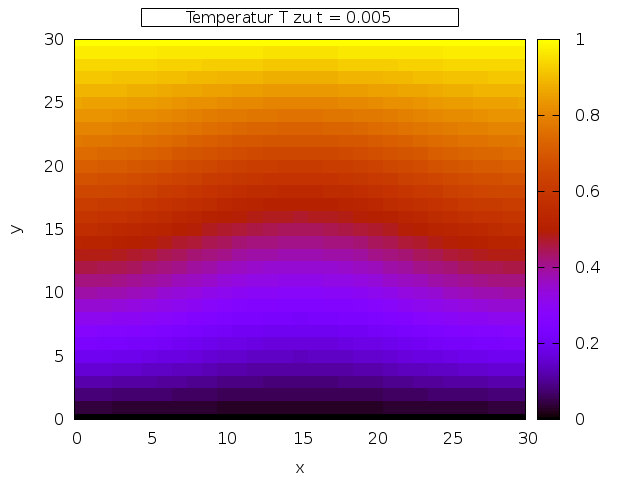
\includegraphics[width=\linewidth]{res/task4/2_0005.png}
   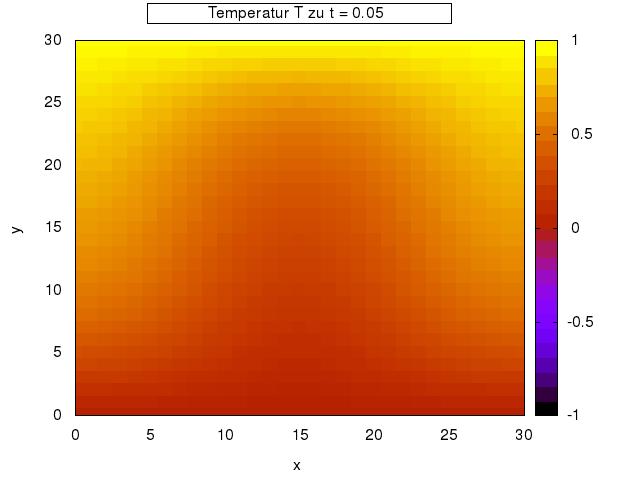
\includegraphics[width=\linewidth]{res/task4/2_005.png}
   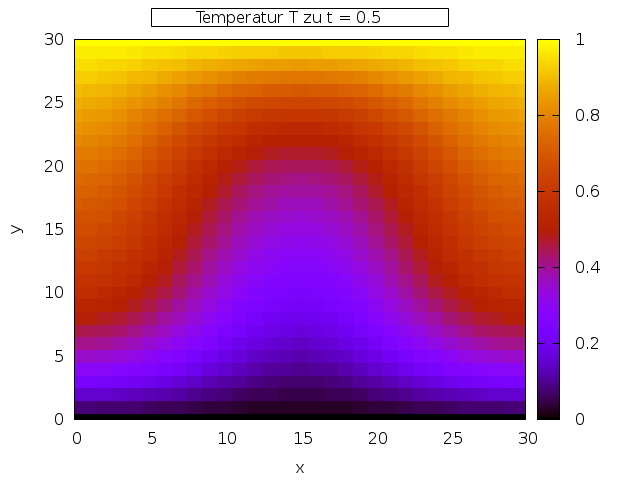
\includegraphics[width=\linewidth]{res/task4/2_05.png}
   \caption{Temperatur für $Pe = 2$.}
   \label{fig:task4_2}
   \end{figure}
   \vspace{1cm}
\end{minipage}%
\hfill%
\noindent\begin{minipage}[t]{0.50\textwidth}% adapt widths of minipages to your needs
\begin{figure}[H]  
   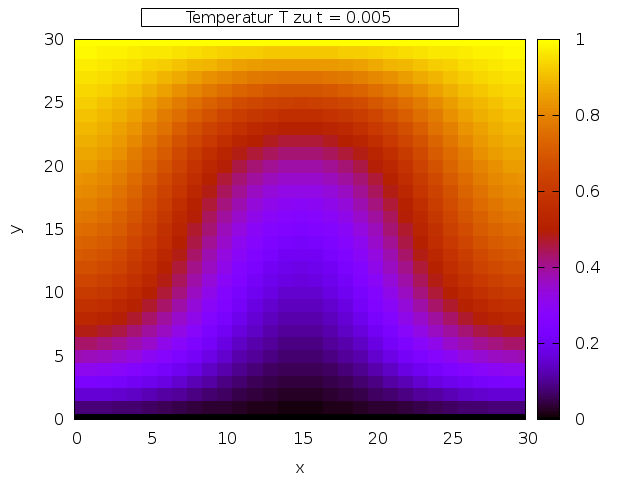
\includegraphics[width=\linewidth]{res/task4/10_0005.png}
   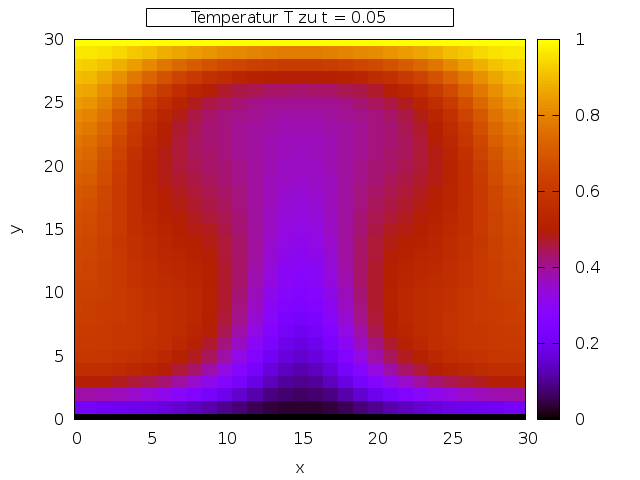
\includegraphics[width=\linewidth]{res/task4/10_005.png}
   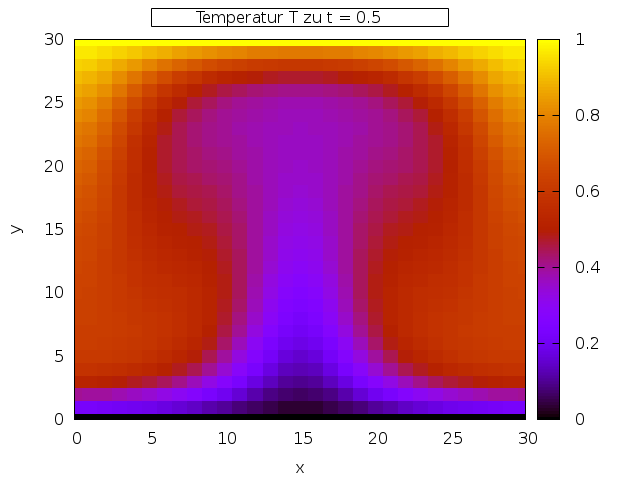
\includegraphics[width=\linewidth]{res/task4/10_05.png}
   \caption{Temperatur für $Pe = 10$.}
   \label{fig:task4_10}
   \end{figure}
\end{minipage}%
\hfill%



\subsection{Aufgabe 5: Beurteilung der Stabilität der FTCS-Lösung}
\label{sec:task5}
Um weitere Aussagen über die numerische Lösung treffen zu können, wird nun noch die Stabilität betrachtet. Hierfür wird zuerst für $N=N_x=N_y = 30$ die maximale Zeitschrittgröße $\Delta t^{Pe}_{max}$ für die \textit{Péclet-Zahlen} $Pe \in \{0.1, 1.0, 10\}$ empirisch ermittelt.\\
Diese ergeben sich zu
\begin{align*}
\Delta t^{0.1}_{max} &= 2.788 \cdot 10^{-4}, \\
\Delta t^{1.0}_{max} &= 2.789 \cdot 10^{-4}, \\
\Delta t^{10}_{max}  &= 2.795 \cdot 10^{-4} .
\end{align*}
Dies liefert einen ersten Eindruck: Die Stabilitätsgrenze hängt von $Pe$ ab, und steigt für steigende $Pe$ in gewissen, geringen Maßen in dem hier betrachteten Intervall an.\\
Für eine genauere Aussage wird nun eine \textit{von-Neumann-Stabilitätsanalyse} durchgeführt. Hierfür wird für die Lösung ein Ansatz der generellen Form
\begin{align*}
T^N_{i,j} = \xi^N e^{i(k_x \Delta x \cdot i + k_y \Delta y \cdot j)}
\end{align*}
gewählt.
Durch Einsetzen in Gleichung (\ref{eq:ftcs}) und Kürzen ergibt sich der Ausdruck
\begin{align*}
\vec{\xi} = 1 &- \frac{\Delta t Pe v^x}{2 \Delta x} \left( e^{i k_x \Delta x} - e^{-i k_x \Delta x} \right) - \frac{\Delta t Pe v^y}{2 \Delta y} \left( e^{i k_y \Delta y} - e^{-i k_y \Delta y} \right) -\frac{2 \Delta t}{\Delta x^2} - \frac{2 \Delta t}{\Delta y^2} \\
 &+ \frac{\Delta t}{\Delta x^2} \left( e^{i k_x \Delta x} + e^{-i k_x \Delta x} \right) +\frac{\Delta t}{\Delta y^2} \left( e^{i k_y \Delta y} + e^{-i k_y \Delta y} \right),
\end{align*}
welcher durch trigonometrische Identitäten in
\begin{align*}
\vec{\xi} = 1 - i \Delta t Pe\left(\frac{ v^x }{\Delta x} \sin(k_x \Delta x) + \frac{v^y}{\Delta y}  \sin(k_y \Delta y) \right) + \frac{2 \Delta t}{\Delta x^2}\cos(k_x \Delta x) &+ \frac{2 \Delta t}{\Delta y^2}\cos(k_y \Delta y) \\ &-\frac{2 \Delta t}{\Delta x^2} - \frac{2 \Delta t}{\Delta y^2}
\end{align*}
übergeht. Damit das Verfahren konvergiert, muss $|\vec{\xi}|$ kleiner $1$ ein. Nähert man hier den Sinus und den Cosinus mit den Maximalwerten, und schätzt die Komponenten $v^x$ und $v^y$ nach oben durch $\pi$ und $2\pi$ ab, so ergibt sich
\begin{align}
\lambda^2 \left(64 + (2 \pi Pe \Delta x)^2 \right) -16 \lambda <0,
\end{align}
mit der \textit{CFL-Zahl} $\lambda = \Delta t/\Delta x^2$.
Eine Lösung dieser Ungleichung ergibt folgenden Bereich, sodass das \textit{FTCS-Schema} konvergiert:
\begin{align}
0 < \lambda = \frac{\Delta t}{\Delta x^2} < \frac{4}{16 + (\Delta_x Pe \pi)^2}.
\end{align}
Hierdurch kann der maximale Zeitschrit, für den das Verfahren konvergiert durch
\begin{align}
\label{eq:neumann_delta_t_max}
\Delta t_{max} = \frac{4 \Delta x^2}{16 + \left(\pi Pe \Delta_x \right)^2}
\end{align}
ausgedrückt werden.

\begin{table}[H]
\centering
	\begin{tabular}{c|c|c}
		\textit{Péclet}-Zahl & $\Delta t_{max}$ (empirisch) & $\Delta t_{max}$ (theoretisch) \\ 
		\hline 
		\hline 
		0.1 & $2.788 \cdot 10^{-4}$  & $2.778 \cdot 10^{-4}$ \\ 
		\hline 
		1 & $2.789 \cdot 10^{-4}$ & $2.776 \cdot 10^{-4}$ \\ 
		\hline 
		10 & $2.795 \cdot 10^{-4}$ & $2.600  \cdot 10^{-4}$ \\ 
		\hline 
	\end{tabular} 
	\caption{Vergleich der empirischen und theoretischen abgeschätzten Werte für $\Delta t_{max}$.}
	\label{tab:delta_t_comp}
\end{table}

Ein Vergleich zwischen den empirisch ermittelten Grenzzeitschritten und den maximalen Zeitschritten, für die nach der nach oben abgeschätzten theoretischen Betrachtung noch ein konvergentes Verhalten zu erwarten ist, bietet die Tabelle (\ref{tab:delta_t_comp}) Es ist zu erkennen, die theoretische Abschätzung für die kleinste \textit{Péclet}-Zahl die beste Übereinstimmung mit dem empirisch gefunden Wert hat - dies hebt den Charakter der bei der Herleitung angenommenen Abschätzungen hervor.  
\\


\newpage
\subsection{Aufgabe 6: BTCS-Lösung}
\label{sec:task6}
Nachdem zuvor die explizite Diskretisierung untersucht wurde, wird das Problem nun implizit im \textit{BTCS-Schema} betrachtet (siehe \ref{sec:btcs}). Dazu werden im Hauptprogramm im Quellcode (2) vier Routinen benötigt.
Die \textit{main}-Methode liest die eingegebene Parameter erneut ein (Zeile 50-88), und befüllt die zuvor eingeführte Matrix $\textbf{M}$. Dazu wird ein Objekt der Klasse \textit{square\_matrix} aus Quellcode (3) benutzt (Zeile 90-155). Diese erbt von der Klasse \textit{matrix}, welche im Quellcode (4) und (6) definiert wird. Hierbei werden die Routinen \textit{beta} und \textit{gamma} benutzt, welche die so benannten Variablen für den jeweiligen Gitterpunkt berechnen (Zeile 21-48). Weitergehend wird das Temperaturfeld nicht mehr in einem zwei sondern in einem eindimensionalen Objekt gespeichert. Dieses wird zunächst mit den gewünschten Startwerten initialisiert (Zeile 155-170).\\
Nun wird über das zu betrachtende Zeitintervall iteriert, und in jedem Integrationsschritt die zuvor aufgestellte Matrix invertiert. Dafür wurde das \textit{SOR-Verfahren} im Quellcode (7) und (5) nach Gleichung (\ref{eq:sor}) implementiert. Dabei werden in jedem einzelnen Interationsschritt die Residuen $\vec{r} = \textbf{M} \vec{x}-\vec{b}$ für die Lösung von $\textbf{M} \vec{x} = \vec{b}$ berechnet, und gefordert, dass der Betrag dieser kleiner als $|\vec{r}| < 10^{-4}$ ist. Dies wird als Abbruchbedingung im dem \textit{SOR-Verfahren} genutzt. Um die Vorteile des \textit{SOR} wirklich nutzen zu können, muss zuerst ein geeigneter Relaxationsparameter $\alpha$ ermittelt werden. Hierzu wird $Pe=10$, $N_x=N_y = 30$ und $\Delta t=100$ gesetzt. Nun wird $\alpha$ mit einer Schrittweite von $0.05$ ab $1.0$ variiert und die benötigten Iterationen ermittelt. 
\begin{figure}[H]
 \centering
   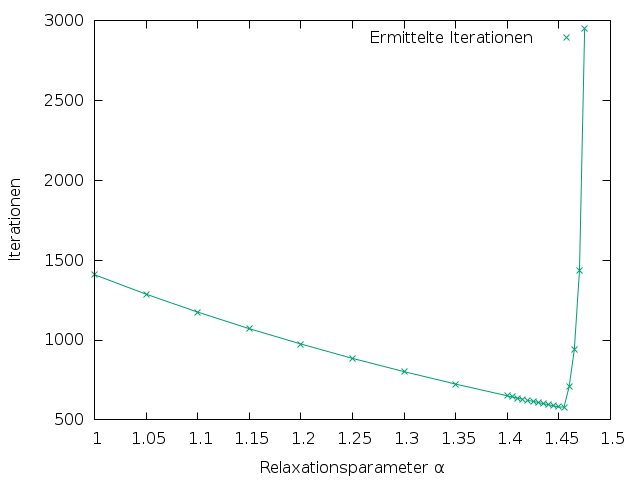
\includegraphics[width=0.65\textwidth]{res/task6/sor_parameter.png}
   \caption{Grafische Darstellung der benötigten Iterationen zur Konvergenz in Abhängigkeit vom Relaxationsparameter $\alpha$.}
 \label{fig:task6_param_comp}
\end{figure}

\noindent\begin{minipage}[t]{0.45\textwidth}% adapt widths of minipages to your needs
\vspace{1cm}
Die grafische Auftragung der so ermittelten Ergebnisse ist in Abbildung (\ref{fig:task6_param_comp}) zu finden. Es ist gut erkennbar, dass das bei $\alpha=1.455$ die geringste Anzahl an Iterationen benötigt wurde. Die Anzahl der benötigten Iterationen für höhere Relexationsparameter $\alpha$ sind nicht mehr graphisch dargestellt, da hier für leicht erhöhte Werte bereits mehrere Zehntausend Iterationen benötigten wurden. Somit wird im weiteren Verlauf dieser Parameter genutzt.\\
Schließlich wird das zuvor implementierte und getestete Verfahren noch einmal für die Parameterwahl aus Aufgabenpunkt (\ref{sec:task4}) angewendet, um die Ergebnisse miteinander zu vergleichen. Hierfür wurde also erneut $Pe = 10$, $\Delta t = 2 \cdot 10^{-4}$ und $t \in \{0.005, 0.05, 0.5\}$ gewählt. Die hierdurch erhaltenen Temperaturverteilungen sind erneut als Heatmap in Abbildung (\ref{fig:task6}) dargestellt.
\end{minipage}%
\hfill%
\noindent\begin{minipage}[t]{0.55\textwidth}% adapt widths of minipages to your needs
\begin{figure}[H]  
   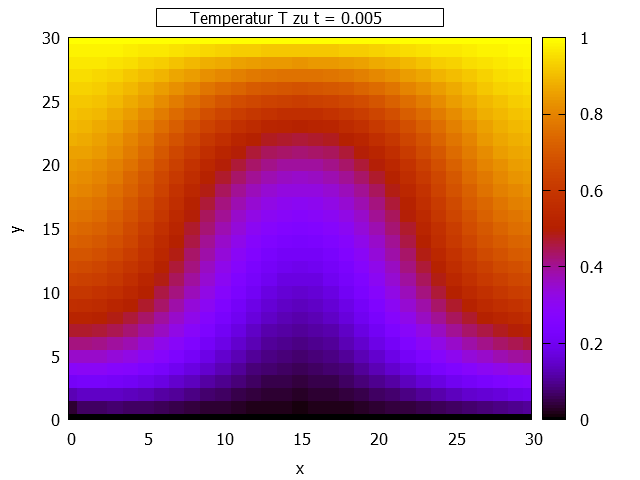
\includegraphics[width=\linewidth]{res/task6/grid0005.png}
   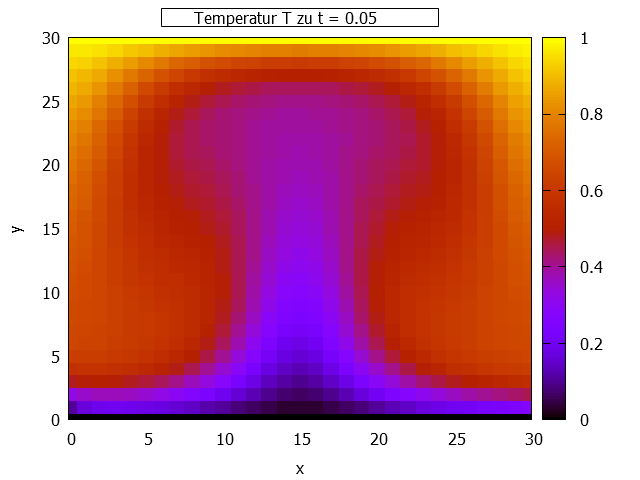
\includegraphics[width=\linewidth]{res/task6/grid005.png}
   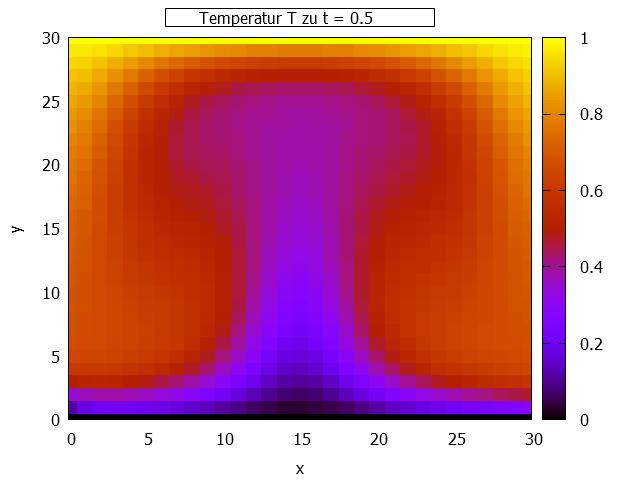
\includegraphics[width=\linewidth]{res/task6/grid05.png}
   \caption{Temperatur nach dem \textit{BTCS-Schema} für $Pe=10$ und $\Delta t = 2\cdot10^{-4}$.}
   \label{fig:task6}
   \end{figure}
\end{minipage}%
\hfill%

\section{Auswertung der Ergebnisse}
\label{sec:interpretation}
\subsection{Numerische Korrektheit der FTCS-Lösung}
\label{sec:disc_num_corr}
Durch den Vergleich in Abschnitt (\ref{sec:task3}) ist erkennbar, dass der numerische Fehler für größere Gitter deutlich geringer wird. Dieser Abfall hat allerdings auch eine bestimmte Grenze. Überschreitet $N = N_x = N_y$ diesen Wert, so kann die numerische Lösung nicht mehr konvergieren. Den Grund für dieses Verhalten (Abweichung der \textit{CFL-Zahl}) ist in Abschnitt (\ref{sec:task5}) beschrieben und erklärt. Anzumerken ist noch, dass der Fehler noch rapider gefallen wäre, wenn man den Gesamtfehler durch die Anzahl der zu berechnenden Gitterpunkte zwecks einer Normalisierung geteilt hätte.

\subsection{Aufgabe 5: Beurteilung der Stabilität der FTCS-Lösung}
\label{sec:disc_stability}
Die zuvor in Abschnitt (\ref{sec:task5}) hergeleitete Gleichung für den maximal gültigen Zeitschritt $\Delta t_{max}$ ist durch die Abschätzungen nach oben, eine obere Schranke. Liegt $\lambda$ außerhalb des Bereiches, aber nahe an der Grenze, so ist ein Konvergieren nicht sicher ausgeschlossen. Liegt $\lambda$ allerdings in dem Bereich, so konvergiert das Verfahren sicher. Dieses Verhalten konnte an den zuvor empirisch ermittelten Grenzen für $\Delta t$ verifiziert werden. Hierbei zeigte sich allerdings, dass die Aussagen der Gleichung (\ref{eq:neumann_delta_t_max}) für geringe \textit{Péclet-Zahlen} zu stark sind, und noch zu viele Werte ausschließen, für die das Verfahren noch konvergiert. Allerdings konnte durch exemplarische Tests bei höheren Werten ein Verhalten festgestellt werden, welches dem durch die Formel beschriebenen entspricht: je höher die Zahl wird, desto feiner muss die Zeitintegration gewählt werden.

\subsection{Aufgabe 6: Auswertung und Vergleich der BTCS-Lösung}
\label{sec:disc_speed_comparison}
Nachdem nun beide Verfahren umgesetzt und getestet worden sind, folgt nun ein Vergleich dieser. Hierbei werden zuerst die dadurch erhaltenen Lösungen miteinander verglichen. Betrachtet man die Ergebnisse für die \textit{Péclet}-Zahl $Pe = 10$ des \textit{BTCS}-Verfahrens aus Abbildung (\ref{fig:task6}) mit denen des \textit{FTCS}-Verfahrens in Abbildung (\ref{fig:task4_10}), so kann man eine hohe Übereinstimmung des Verlaufes festellen. Hierbei ist für diese gegebene Parameterwahl kein Unterschied feststellbar.
\begin{table}[H]
	\centering
	\begin{tabular}{c|c|c}
		Simulierte Zeitspanne $t$ & \textit{FTCS} [sec] & \textit{BTCS} [sec] \\ 
		\hline  \hline 
		1 & $<$ 1 & 6 \\ 
		\hline 
		10 & 3 & 7 \\ 
		\hline 
		50 & 15 & 8 \\ 
		\hline 
		100 & 33 & 9 \\ 
		\hline 
		200 & 68 & 9 \\ 
		\hline 
		400 & 135 & 10 \\ 
		\hline 
	\end{tabular}
	\label{table:speed_comparison} 
	\caption{Exemplarischer Laufzeitvergleich zwischen dem expliziten (\textit{FTCS}) und dem impliziten (\textit{BTCS}) Lösungsverfahren.}
\end{table}
Da zuvor das explizite Lösungsverfahren auf numerische Korrektheit überprüft wurde, kann also auch davon ausgegangen werden, dass das implizite Lösungsverfahren korrekt umgesetzt worden ist.\\
Betrachtet man allerdings die Laufzeit der beiden Verfahren, so können große Unterschiede sowohl in der Größenordnung, als auch im Verlauf festgestellt werden. Diese Laufzeiten wurden exemplarisch gemessen und in Tabelle (\ref{table:speed_comparison}) festgehalten. Es ist anzumerken, dass die gemessene Laufzeit von dem verwendeten Rechner und anderen äußeren Einflüssen abhängen kann, sodass diese Daten nur als Anhaltspunkt für das grobe Verhalten gesehen werden können. Zudem hätten die verschiedenen Routinen auch noch weiter hinsichtlich ihrer Laufzeit optimiert werden können. Da dies den Rahmen des Themas der Arbeit überschreiben würde, wurde darauf verzichtet.\\
Es ist zu erkennen, dass die Laufzeit des expliziten Verfahrens in etwa linear mit der simulierten Zeitspanne $t$ anwächst, wohingegen die des impliziten Verfahrens deutlich geringer anwächst, und näherungsweise fast konstant bleibt.\\
Somit zeigt sich, dass das explizite Verfahren zweiter Ordnung in diesem Fall seine Stärken nur bei sehr kurzen Zeitspannen hat. Das implizite Verfahren läuft bereits bei Simulationen für mehr als $t=50$ schneller ab.

\begin{thebibliography}{9}
  \bibitem{manmana}
  Andres Honecker, Thomas Pruschke, Salvatore R. Manmana, \\
  \emph{Scriptum zur Vorlesung: Computergestütztes wissenschaftliches Rechnen}. \\
 Göttingen,
  Sommersemester 2016

  \bibitem{sor}
  W. Auzinger, \\
  \emph{Lecture Notes Iterative Solution of Large Linear Systems}. \\
 Wien, 2011
 
   \bibitem{per}
  F. Peric, \\
  \emph{Computational Methods for Fluid Dynamics}. \\
 Stanford, 2002
 
 
 
 \end{thebibliography}
\clearpage

\clearpage

\appendix
\section{Quellcode}
\subsection{Hauptprogramme}
\label{sec:source_main} 
\lstinputlisting[label={src:ftcs}, title=\textbf{Quellcode 1:} Implementation des FTCS-Schemas]{source/ftcs.cpp}
\lstinputlisting[label={src:btcs}, title=\textbf{Quellcode 2:} Implementation des BTCS-Schemas]{source/btcs.cpp}

\clearpage

\subsection{Hilfsbibliotheken}
\label{sec:source_lib} 
\lstinputlisting[label=src:squarematrix.h, title=\textbf{Quellcode 3:} square\_matrix.h]{source/lib/square_matrix.h}
\lstinputlisting[label=src:matrix.h, title=\textbf{Quellcode 4:} matrix.h]{source/lib/matrix.h}
\lstinputlisting[label=src:linearsystem.h, title=\textbf{Quellcode 5:} linear\_system.h]{source/lib/linear_system.h}

\lstinputlisting[label=src:matrix.cpp, title=\textbf{Quellcode 6:} matrix.cpp]{source/lib/matrix.cpp}
\lstinputlisting[label=src:linearsystem.cpp, title=\textbf{Quellcode 7:} linear\_system.cpp]{source/lib/linear_system.cpp}
\end{document}